\section{Cultivation and differentiation of HAoSMCs}
\label{sec:cultivation}
\Acp{haosmc} were used for the following experiments.. This cell type is commonly used to study of cardiovascular function and disease \cite{[Reference for this claim]}. Cells were kept at 37\,°C and 5\,\% \ac{co2} whenever possible. For differentiation, cells were first treated with \ac{tgf} to induce a contractile phenotype. Afterward, \acp{haosmc} were stimulated with \acf{il1} and \ac{pdgf} to induce a synthetic or pro-inflammatory phenotype. Please refer to sections \ref{sec:tgf} and \ref{sec:pdgf} and the referenced literature for more information.

    \subsection{Thawing and Cultivation}
    For longtime storage, cells were stored in liquid nitrogen. New cells (\nth{6} passage) were thawed at 37\,°C in the water bath and transferred to a 15\,mL tube when required. After centrifugation for two\,min at 300\,xg, the supernatant was discarded. The cell pellet was taken up in 14\,mL of \ac{M231} + \ac{smgs} for cultivation in a TC Flask T75. Every other day, 2/3 of the medium was removed and replaced by fresh. Cells were cultivated to a maximum passage of 10.

    \subsection{Passaging}
    \acp{haosmc} were passaged at a maximum of 80\,\% confluency (approximately once a week). The medium was removed, and cells were washed once with 5\,mL of \ac{pbs}. Washed cells were incubated with 3\,mL trypsin for 4\,min at 37\,°C. The trypsin was inactivated by adding 7\,mL \ac{M231}. Subsequently, the cell suspension was transferred to a 15\,mL tube and pelleted for 4\,min at 300xg. Finally, the supernatant was removed and the pellet resuspended in \ac{M231} supplemented with \ac{smgs}. The cells were seeded with a density of ~$\num{500e3}$ \acp{haosmc} per TC Flask T75.

    \subsection{Preparation of Collagen I matrix}
    \label{subsec:matrix}
    The \ac{col1} matrix (1.8\,mg/mL) was prepared by mixing the components according to table \ref{tab:matrix}. All components were stored at 4\,°C, and all pipetting steps were carried out on ice:

    \begin{table}[h]
    \capstart
	\centering
	\begin{minipage}{\captionwidth}
	   	\caption[Col I matrix]{\uzlemph{\ac{col1} Matrix Composition}}
	   	\label{tab:matrix}
	\end{minipage}
    \begin{tabular}{|l|l|r|}
        \hline
        component & concentration & volume (µL) \\ \hline
        \ac{water}       & -             & 38.9        \\
        \ac{M231}      & -             & 53.3        \\
        \ac{smgs}      & 20x           & 5,3         \\
        NaOH      & 1 M           & 2,7         \\
        NaHCO3    & 7.5 \%        & 2.1         \\
        \ac{col1}    & 5 mg/mL       & 57.6        \\ \hline
        total     & -             & 160         \\ \hline
    \end{tabular}
    \end{table}

    160\,µL of matrix mix were transferred in each well of a \ac{24 well}. For polymerization, the matrix was incubated at 37\,°C for 60\,min.

    \subsection{Differentitation of HAoSMCs}
    \label{subsec:differentiation}
    Differentiation was carried out over seven days in \acp{24 well}. Differentiation was carried out in 1\,mL M231 supplemented with 1\,\% \ac{fbs}, and the indicated cytokines:
    \begin{itemize}
        \item \textbf{Day 0:} Matrix and cells were prepared as described in the previous section. Seeding of $\num{40e3}$ in \ac{M231} + \ac{smgs} on 160\,µL \ac{col1} matrix or the Nunclon\texttrademark~Delta well.
        \item \textbf{Day 1:} The medium was replaced with 1\,mL M231 + 1\,\% \ac{fbs} + 5\,ng/mL \ac{tgf}
        \item \textbf{Day 5:} The medium was replaced with 1 mL M231 + 1\,\% \ac{fbs} + 10\,ng/mL \ac{il1} + 10\,ng/mL \ac{pdgf}
        \item \textbf{Day 7:} Potential additional assay-specific stimulation.
    \end{itemize}
    Controls were run alongside without cytokines.

\section{mRNA Quantification}
\label{sec:qpcr}
SYBR\textregistered~Green is an intercalating \ac{dna} dye that allows for the monitoring of \ac{dna} amplification. Fluorescence is measured after every amplification cycle of the \ac{pcr}. A lower \ac{Cq} corresponds to a higher initial \ac{dna} concentration. \cite{huggettStandardisationReportingNucleic2011}\\
\Ac{qpcr} was utilized to assess the \ac{mRNA} concentration of the two reporter genes \ac{cnn1} and \ac{mmp9} in differentiated \acp{haosmc}. The housekeeping gene \ac{gapdh} was used as a reference.


    \subsection{\ac{rna} Isolation}
    \ac{rna} was isolated using the Total \ac{rna} Purification Kit. The extraction was performed according to the manufacturer's protocol, using the optional washing step with 700\,µL 80\,\% ethanol, and \ac{rna} was eluted with 30\,µL of RNase-free water.

    \subsection{Reverse Transcription}
    For \ac{RT}, \ac{rna} samples were diluted to yield 10\,µL of 10\,ng/µL. The \ac{rna} was heated for 5\,min at 68\,°C. Afterward, 10\,µL of the \ac{RT} reaction mix was added:

    \begin{table}[h]
    \capstart
	\centering
	\begin{minipage}{\captionwidth}
	   	\caption[RT mastermix]{\uzlemph{Reaction Mix for RT}}
	   	\label{tab:RT Mastr Mix}
	\end{minipage}
    \begin{tabular}{|l|l|r|}
        \hline
        component               & concentration & volume (µL) \\ \hline
        First Strand Buffer     & 5x            & 4           \\
        \acs{DTT}               &\textbf{\color{red} ?!?}               & 2           \\
        \acs{dNTP}              &\textbf{\color{red} ?!?}               & 1           \\
        Oligos                  &\textbf{\color{red} ?!?}               & 1           \\
        RiboLock                &\textbf{\color{red} ?!?}               & 1           \\
        M-MLVRT                 &\textbf{\color{red} ?!?}               & 1           \\ \hline
    \end{tabular}
    \end{table}

    \ac{RT} was carried out for 60\,minutes at 37\,°C before inactivating the enzyme for 5\,minutes at 95\,°C. \Ac{cDNA} was either used for \ac{qpcr} or stored at -20\,°C.

    \subsection{qPCR}
    \begin{table}[h]
    \capstart
	\centering
	\begin{minipage}{\captionwidth}
	   	\caption[qPCR samples]{\uzlemph{Sample Composition for qPCR}}
	   	\label{tab:qPCR_MM}
	\end{minipage}
    \begin{tabular}{|l|l|r|}
        \hline
        component                  & concentration & volume (µL) \\ \hline
        SYBR GREEN Master Mix      & 1:2          & 3.75        \\
        Primer (forward + reverse) & 5 pM (each)  & 1.125       \\
        \ac{water}                        & -            & 1.125       \\
        \ac{cDNA}                       & -            & 1.5           \\ \hline
    \end{tabular}
    \end{table}
    Samples were prepared in a 384-well Multiply \ac{pcr} plate. Wells were sealed and thoroughly mixed by invertation of the plate. The assay was performed with a 7900HT Fast Real-Time \ac{pcr} System:

    \begin{table}[h]
    \capstart
    \centering
    \begin{minipage}{\captionwidth}
        \caption[qPCR programme]{\uzlemph{qPCR Cycle}}
        \label{tab:qPCR_programme}
    \end{minipage}
    \begin{tabular}{|c|r|c|c|r|}
    \hline
        step & time (s) & temperature (°C) & loop to & passes \\ \hline
        1    & 120      & 50               &         & 1      \\
        2    & 600      & 95               &         & 1      \\
        3    & 15       & 60               &         & 40     \\
        4    & 60       & 60               & 3       & 40     \\
        5    & 600      & 95               &         & 1      \\
        6    & -        & 16               &         & 1      \\ \hline
    \end{tabular}
    \end{table}

    \subsection{Processing of Data}
    The \ac{Cq} was automatically calculated by the software SDS2.2.2. The arithmetic mean of three technical replicates was calculated for each sample, disregarding values that are apparent outliers. For normalization, the mean \ac{Cq} of the reference gene \ac{gapdh} was subtracted from the mean \ac{Cq} of the gene of interest:

    $$\Delta ct = ct(\mathrm{gene of interest}) - ct(\mathrm{GAPDH})$$

    Taking into account the exponential amplification of \ac{dna} in \ac{pcr}, the $\Delta ct$ can then be transformed into a relative expression level. Where $\num{10e6}$ is a constant to yield readable values:

    $$\mathrm{rel. expr.} = 2^{-\Delta ct\num{10e6}}$$

    In total, four biological replicates were performed. Data visualization and statistical analysis were carried out in python. A student's t-test was used for statistical testing, and a p-value of 0.05 is considered significant. For detailed information, please refer to the script.

\section{Energy Profiling}
\label{sec:seahorse}
The Seahorse XF Analyzer allows real-time measurement of dissolved oxygen and protons in a confined small volume using solid-state sensor probes. The measurements are then used to calculate a cell monolayer's \ac{ocr} and \ac{ecar}. The \ac{ocr} and \ac{ecar} are indicators for mitochondrial respiration and glycolysis. They can be used to assess the metabolic state of cells. \cite{agilenttechnologiesHowAgilentSeahorse2022}\\
Seahorse assay was utilized to assess the energy profile of differentiated \acp{haosmc}. For this assay, cells were not differentiated in a \ac{24 well} but XF24 Cell Culture Microplates. Since the confined volume required for the assay would not fit the matrix, cells were not cultivated on \ac{col1}!

    \subsection{Seahorse Assay}
    On the day before the assay, the Seahorse XF Analyzer was set up to calibrate. The XF24 Extracellular Flux Assay Kit cartridge was equilibrated in Seahorse XF calibrant overnight at 37\,°C in a non-\ac{co2} environment.\\
    On the day of the assay, \acp{haosmc} were washed with 500\,µL PBS each. Afterward, the XF BASE medium was supplemented with 1\,mM sodium pyruvate, 10\,mM glucose, 2\,mM glutamine, and 90\,µM NaOH. Cells were incubated for 1\,h at 37\,°C in a non-\ac{co2} environment with supplemented 500\,µL XF BASE medium. Toxins for disruption of the respiratory chain were prepared and loaded into the XF24 Extracellular Flux Assay cartridge:

    \begin{table}[h]
    \capstart
    \centering
    \begin{minipage}{\captionwidth}
        \caption[toxins for seahorse]{\uzlemph{Toxin Concentrations for XF24 Extracellular Flux Assay}}
        \label{tab:seahorse_toxins}
    \end{minipage}
    \begin{tabular}{|l|r|r|r|}
        \hline
        component  & concentration in cartridge (µM) & volume in cartridge (µL) & concentration in well (µM) \\ \hline
        Oligomycin & 14                             & 55                      & 1.4                        \\
        FCCP       & 10                             & 60                      & 2.0                        \\
        Antimycin  & 50                             & 65                      & 5.0                        \\ \hline
    \end{tabular}
    \end{table}

    The cartridge was mounted into the XF Analyzer for calibration. After successful calibration, the hydration cartridge was replaced with the cell plate. The measurement was programmed as the following:

    \begin{itemize}
        \item Calibration of the probes.
        \item Equilibration
        \item 3 Repeats of:
        \begin{itemize}
            \item Mixing (1\,min)
            \item Pause (2\,min)
            \item Detection of \ac{ocr} and \ac{ecar} (4\,min)
        \end{itemize}
        \item Pause (2\,min)
        \item Injection of 55\,µL Oligomycin
        \item 3 Repeats of:
        \begin{itemize}
            \item Mixing (1\,min)
            \item Pause (2\,min)
            \item Detection of \ac{ocr} and \ac{ecar} (4\,min)
        \end{itemize}
        \item Pause (2\,min)
        \item Injection of 60\,µL FCCP
        \item 3 Repeats of:
        \begin{itemize}
            \item Mixing (1\,min)
            \item Pause (2\,min)
            \item Detection of \ac{ocr} and \ac{ecar} (4\,min)
        \end{itemize}
        \item Pause (2\,min)
        \item Injection of 55\,µL Antimycin
        \item 3 Repeats of:
        \begin{itemize}
            \item Mixing (1\,min)
            \item Pause (2\,min)
            \item Detection of \ac{ocr} and \ac{ecar} (4\,min)
        \end{itemize}
    \end{itemize}

    After the measurement, the medium was removed, and \acp{haosmc} were stained for 15\,min with 1\,µg/mL Hoechst 33342 in \ac{pbs}. Finally, the cells were imaged to determine cell count for normalization.

    \subsection{Processing of Data}
    \begin{figure}[h]
    \capstart
        \centering
        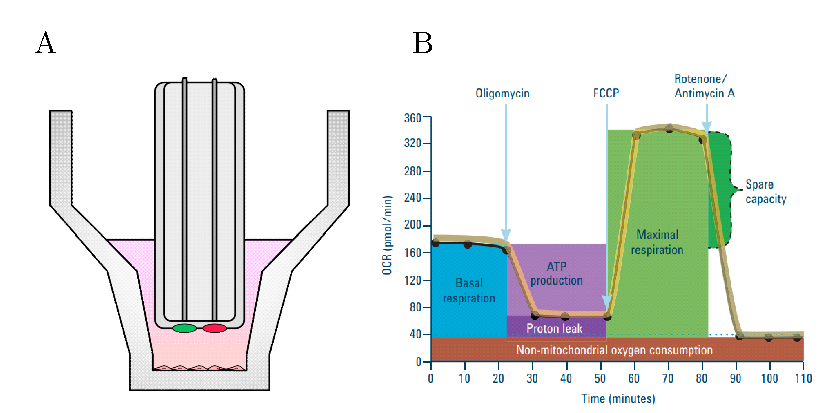
\includegraphics{Abbildung/seahorse_basics_placeholder.pdf}

        \begin{minipage}{\captionwidth}
            \caption[enrichment]{\uzlemph{Basics of Seahorse Assay}\\
            \textbf{(A)} Schematic of a well used in Seahorse Assay. For the measurement, the piston in the middle lowers to the bottom, defining a restricted space at the bottom. \ac{ocr} and \ac{ecar} in this volume are measured via two probes (red and green). \textbf{(B)} Exemplary curve for \ac{ocr} recorded over time and extractable properties of the respiratory chain \cite{AGILENT WEBSITE; ADD SOURCE}.}
            \label{fig:seahorse_basics}
        \end{minipage}
    \end{figure}

    Cells were quantified using a python script provided by Dr. Tobias Reinberger. \ac{ocr} and \ac{ecar} were calculated with Wave Controller, which were normalized using the cell count and the signal in the control wells. In total, three biological repeats were recorded. One repeat was excluded because no changes in \ac{ocr} and \ac{ecar} could be detected and cells detached from the bottom of the wells. One of the five technical repeats for each condition was manually excluded for the remaining replicates. Further, initial \ac{ocr} and \ac{ecar}, as well as the characteristics of the respiratory chain displayed in figure \ref{fig:seahorse_basics} B, were calculated using a modified python script provided by Dr. Tobias Reinberger. Welch’s t-test was used for statistical analysis, and a p-value of 0.05 is considered significant. For detailed information, please refer to the script.

\section{Oxidative Stress Assay}
\label{sec:cellrox}
CellROX\texttrademark~Green is a fluorescent dye that gets oxidized by elevated levels of \ac{ros}. The oxidized form binds to \ac{dna} and shows bright-green fluorescence \cite{thermofisherscientificinc.CellROXGreenReagent2022}.\\
CellROX\texttrademark~Green assay was used to assess the generation of \ac{ros} in differentiated \acp{haosmc}. After differentiation, further stimulation (from here on referred to as \textit{boost}) with \ac{pdgf} was carried out. Finally, a recovery experiment was performed using \ac{nac}. \ac{nac} is a potent antioxidant.

    \subsection{CellROX\texttrademark~Assay}
    For the assay, cells were washed with \ac{pbs}. Then the boost was performed using variable concentrations of \ac{pdgf} in 300\,µL \ac{hbss}. For \ac{ros} quenching with \ac{nac}, 0.25\,M \ac{nac} solution was added to the wells 2\,h prior to the experiment and the \ac{pdgf}-CellROX\texttrademark~Green Mix.

    \begin{table}[h]
    \capstart
    \centering
    \begin{minipage}{\captionwidth}
        \caption[Seahorse Assay]{\uzlemph{Composition of the \ac{pdgf}-CellROX\texttrademark~Green Mix}}
        \label{tab:cellrox_table}
    \end{minipage}
    \begin{tabular}{|l|r|r|r|}
        \hline
        component         & concentration & final concentration      & volume (µL) \\ \hline
        HBSS              & -             & -                        & 300         \\
        PDGF              & 100\,µg/mL             &  (0\,-\,400\,ng/mL) & variable    \\
        Hoechst           & 1\,mg/mL       & 1\,µg/mL                  & 0.3         \\
        CellROX\texttrademark~Green (1:500) & 2.5\,mM        & 5\,µM                     & 0.6         \\
        NAC               & 0.25\,M        &  (0\,-\,8\,mM)      & variable    \\ \hline
        total             & -             & -                        & $\sim$300   \\ \hline
    \end{tabular}
    \end{table}

    During the boost, cells were kept at 37\,°C in a 5\,\% \ac{co2} environment. The boost time (60, 120, 180, or 240\,min) is indicated along the results of the respective experiment. Imaging was done with the BZ-X810 All-in-One Fluorescence Microscope, using standard sensitivity. Images for the \acf{nac} quench were recorded as a z-stack and merged into one image using [KEYENCE SOFTWARE].

    \subsection{Processing of Data}
    \label{subsec:cellrox_data_processing}
    Seven biological repeats were performed for \ac{pdgf}-boost titration. One repeat was excluded because of a high signal in the negative control. Four biological repeats were performed for the \ac{nac} quench, one of which has been excluded because no signal in the positive control could be detected.
    For quantification of signal intensity, pixels with a green value higher than 90 were counted. Differences in cell count were adjusted by dividing the green pixel by the number of blue pixels with a threshold of 80. To adjust for the large variance in total signal intensity between biological repeats, values were normalized by division through the total signal of all recorded conditions.
    The Mann-Whitney U test was used for statistical testing. A p-value of 0.05 is considered significant. For detailed information, please refer to the scripts.


\section{Curation of Data for postGWAS Analyses}
\label{sec:database}
Data for post\ac{gwas} analyses and co-visualization with the \ac{gwas} summary statistics were downloaded from public resources. Processing of the data and further annotation is briefly listed and described below. The generated tables are summarized in figure \ref{fig:db_er} and table \ref{tab:db_tables}. For a complete view, please refer to the download scripts.

\begin{itemize}
    \item \uzlemph{GWAS Summary Statistics:} The \ac{cad} \ac{gwas} summary statistics from \textcite{aragamDiscoverySystematicCharacterization2021} and a list of identified proxy \acp{snp} were annotated via the Ensembl \ac{rest} \ac{api} by Dr. Tobias Reinberger.

    \item \uzlemph{HGNC Gene List} The newest quarterly update to the complete \ac{hgnc} dataset was downloaded via the \MYhref{http://ftp.ebi.ac.uk/pub/databases/genenames/hgnc/archive/}{\ac{hgnc} \ac{ftp} server}. The dataset was generated a list of all 43,135 approved symbols, mapping to their \ac{hgnc} ID. Further, a list of all 98,723 symbols (approved, alias, and previous) mapping to their \ac{hgnc} ID was generated.

    \item \uzlemph{Linked SNPs} \ac{ld} $r^2$ values in a 500 kb window were calculated for the list of \ac{cad} \ac{gwas} proxy variants via the \MYhref{https://rest.ensembl.org/documentation/info/ld_id_get}{Ensembl \ac{rest} \ac{api}}. For humans, Ensembl calculates the \ac{ld} with data from the 1000 Genomes project (see table \ref{tab:populations}). In the same process, linked \acp{snp} were annotated with their most severe consequence from the Ensembl \ac{vep}. In total, information for 449,770 relationships were downloaded.

    \begin{table}[h]
    \capstart
    \centering
    \begin{minipage}{\captionwidth}
        \caption[1000 Genomes Populations]{\uzlemph{1000 Genomes Populations}}
        \label{tab:populations}
    \end{minipage}
    \begin{tabular}{|l|r|r|}
        \hline
        Name                   & Size (individuals)   & Description      \\ \hline
        1000GENOMES:phase3:ALL & 2504                 & All phase 3 individuals  \\
        1000GENOMES:phase3:AMR & 347                  & Americans  \\
        1000GENOMES:phase3:EAS & 504                  & East Asians  \\
        1000GENOMES:phase3:EUR & 503                  & European \\
        1000GENOMES:phase3:SAS & 489                  & South Asian  \\ \hline
    \end{tabular}
    \end{table}

    \item \uzlemph{Ensembl Genome Annotations} The newest Ensembl build (Ensembl release 106) was downloaded via the \MYhref{http://ftp.ensembl.org/pub/current_gtf/homo_sapiens/}{Ensembl \ac{ftp} server}. Features annotated as protein-coding (19,994), \ac{lncRNA} (17,734), or \ac{miRNA} (1,877) genes were extracted. Further, gene symbols were mapped to their \ac{hgnc} ID if possible.

    \item \uzlemph{Ensembl Regulatory Build} The newest Ensembl regulatory build (Ensembl release 106) was downloaded via the \MYhref{http://ftp.ensembl.org/pub/current_regulation/homo_sapiens/}{Ensembl \ac{ftp} server}. The build contains:
    \begin{itemize}
        \item 110,623 open chromatin regions
        \item 30,873 \ac{tf} binding sites
        \item 175,885 \ac{ctcf} binding sites
        \item 127,935 enhancers
        \item 36,597 promotors
        \item 140,548 promotor flanking regions
    \end{itemize}

    \item \uzlemph{Open Target Genetics l2g Scores} The latest list of Open Target Genetics \ac{l2g} Scores was downloaded via the \MYhref{http://ftp.ebi.ac.uk/pub/databases/opentargets/genetics/latest/l2g/}{open target genetics \ac{ftp} server}. Entries were annotated with their \ac{hgnc} ID whenever possible. 655 entries that do not map to a gene approved by the \ac{hgnc} were excluded, yielding a total of 3,580,206 database entries.

    \item \uzlemph{TSS} 35,160 \ac{tss} for protein-coding genes were extracted from a \MYhref{https://ccg.epfl.ch/mga/hg38/gencode/}{\ac{USCS} Genome Browser dump}.

    \item \uzlemph{Associated traits from the GWAS catalog} The \ac{snp} trait associations from the latest release of the GWAS catalog were downloaded via the \MYhref{http://ftp.ebi.ac.uk/'}{GWAS catalog FTP server}. 14,892 \ac{snp}-trait correlations missing a position on the human reference genome or the p-value for the association were excluded from the data set. In total, 370,002 associations from 5,831 distinct studies were collected.

    \item \uzlemph{TADs} \acp{tad} predicted by software adapted from \textcite{dixonTopologicalDomainsMammalian2012} were downloaded via the \MYhref{http://3dgenome.fsm.northwestern.edu/publications.html}{3D genome browser}. In total, \acp{tad} in 40 distinct biosamples were downloaded.

    \item \uzlemph{scATAC-seq from \textcite{newmanMultipleCellTypes2021a}} Processed sc\ac{atac} data for 8 cell types [SOME MORE INFO] were scraped from the \MYhref{https://github.com/MillerLab-CPHG/Coronary_snATAC/tree/main/3_SVMpipeline/celltype_peaks}{Miller Lab GitHub repository}.

    \item \uzlemph{scATAC-seq from CATlas} Processed \ac{sc}\ac{atac} data was scraped from the \MYhref{http://renlab.sdsc.edu/kai/Key_Processed_Data/Peaks/}{Ren Labs website} for 222 biosamples.

    \item \uzlemph{ABC model} The \ac{abc} model data for 131 biosamples was downloaded from the \MYhref{http://ftp.broadinstitute.org/outgoing/lincRNA/ABC/}{Engreitz Lab \ac{ftp} server}. The data was further translated from \ac{hg19} to \ac{hg38} using pyliftover.

    \item \uzlemph{ENCODE cCREs} \acp{cCRE} in distinct biosamples were downloaded by Dr. Tobias Reinberger, filtering out elements annotated as \textit{unclassified}.
\end{itemize}

\section{Visualization of GWAS data}
\label{sec:gwas_vis}
For visualization of the data, a bokeh application was built. The application fetches the data from the database and renders it to a web browser \cite{bokehdevelopmentteamBokehPythonLibrary2022}.\\
Bokeh is a python module that allows easy and interactive visualization of data. It combines the powerful data processing tools of python with the interactivity of \ac{js} running in the browser. The python side of bokeh creates python objects that are serialized into \ac{json} data and handed over to bokehJS. bokehJS deserializes these into \ac{js} objects that are rendered to the browser. The integrated bokeh server additionally allows synchronization of data between the underlying python environment and browser-side \ac{js} library. All in all, allowing real-time updates to the displayed data.

    \begin{figure}[h]
    \capstart
        \centering
    	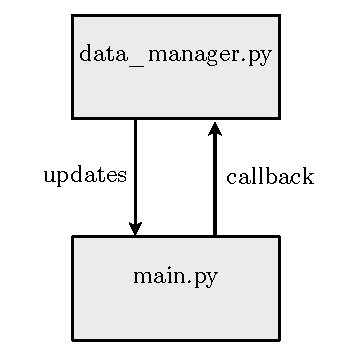
\includegraphics{Abbildung/vis_architecture.pdf}

    	\begin{minipage}{\captionwidth}
    		\caption[vis archi]{\uzlemph{Architecture of the GWAS Navigator}}
    		\label{fig:plot_architecture}
    	\end{minipage}
    \end{figure}

According to good design principles, the concerns of the application are split into two sections, as shown in fig. \ref{fig:plot_architecture}. Reading the data from the database and further processing steps are managed by a data provider and enclosed in one class. In contrast to the model-controller-view architecture, a popular architectural pattern for the design of user interfaces, there is no partition between a view and a controller \cite{langtangenUsingWebFrameworks2015}. Since data visualization and the control widgets are created by bokeh, it is convenient to use the built-in event listeners of the library to handle the required callbacks. Therefore, the main file is responsible for creating all plots and widgets and handling user inputs.

\section{Enrichment analysis}
\label{sec:enrichment}
Based on the data in the database, initial postGWAS studies were run. Annotation enrichment analyses are a popular tool for identifying terms over-represented in a list of interest. The most prominent application is their application as \ac{gsea}. \Acp{gsea} are used to check for the overrepresentation of a candidate gene list in a predefined set of genes \cite{tipneyIntroductionEffectiveUse2010}. In this case, using Fisher's exact test, the method is used to determine whether \acp{cCRE} overlap with \ac{cad}-associated \acp{snp} is enriched in certain biosamples.\\
For the analysis, \acp{cCRE} annotated as unclassified were excluded. As a list of \ac{cad}-associated \acp{snp}, the list of 241 proxy variants from the database was used, as well as all linked variants ($r^2\geq0.6$) in the 1000 Genomes European Population. The following parameters were calculated for all biosamples:

\begin{itemize}
    \item The number of distinct \acp{cCRE} among all biosamples (m)
    \item The number of distinct \acp{cCRE} that are annotated in the biosample of interest (mt)
    \item The Number of distinct \acp{cCRE} that overlap with an SNP in the SNP list in any biosample (n)
    \item The Number of distinct \acp{cCRE} that overlap with an SNP in the SNP list in the biosample of interest (nt)
\end{itemize}

The p-value for the number of overlaps greater than or equal to the observation can be calculated as the cumulative distribution function of the hypergeometric distribution \cite{}.

$$ P(\sigma_t\geq n_t) = \sum_{k=n_t}^{min(m_t, n)} \frac{\binom{n}{k}\binom{m-n}{m_t-k}}{\binom{m}{m_t}} $$

To account for the multiple comparisons problem, p-values were adjusted with Bonferroni correction, where n is the number of tests ($\equiv$ number of biosamples):

$$ p_{ajd.} = p*n$$

The analysis and visualization were done in python. An adjusted p-value of 0.05 is considered significant. Finally, the identified biosamples were annotated via the \MYhref{https://web.expasy.org/cellosaurus/}{cell line database Cellosaurus}. For detailed information, please refer to the analysis scripts.

\begin{figure}[h]
\capstart
    \centering
    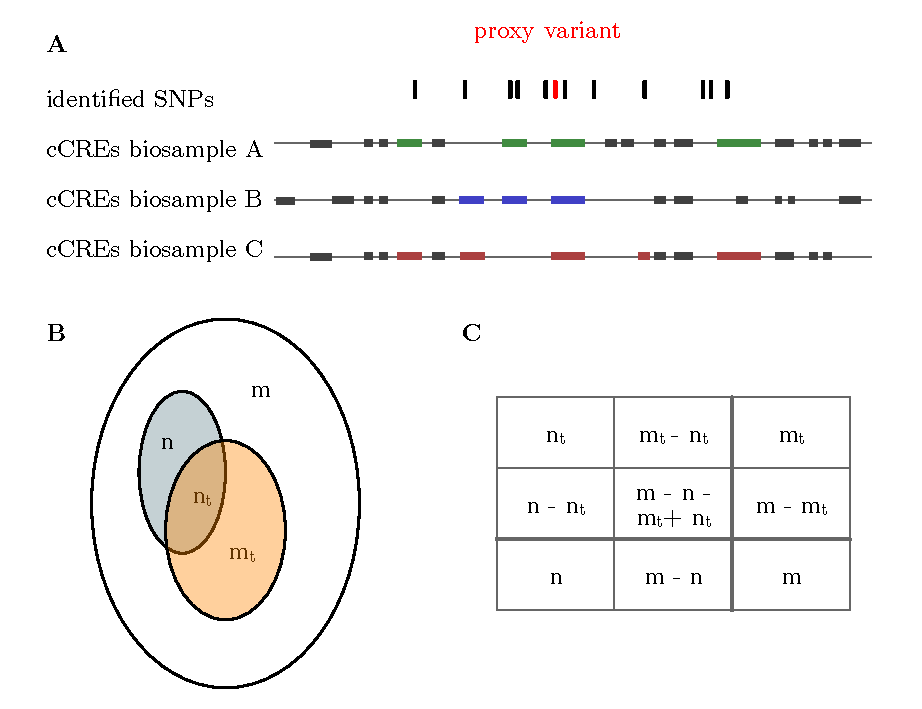
\includegraphics{Abbildung/enrichment.pdf}

    \begin{minipage}{\captionwidth}
        \caption[enrichment]{\uzlemph{Enrichment analysis for \acp{cCRE} overlapping with \ac{cad} risk \acp{snp}}\\
        \textbf{(A)} Visual representation of the overlap calculation for enrichment calculation. The proxy variant is indicated as a red line, variants in \ac{ld} are indicated as black lines. \ac{cCRE} are shown as boxes, those that are overlapping with an \ac{snp} were colored according to the biosample they were annotated in. \textbf{(B)} Venn diagram of these values for a biosample. \textbf{(C)} Schematic contingency table for a biosample. \\
        (m) is the number of distinct \acp{cCRE} found among all biosamples (23 in this example); (mt) the number of distinct \acp{cCRE} annotated in the biosample of interest (16 for biosample A, 14 for biosample b, 14 for biosample C); (n) the number of distinct \acp{cCRE} overlapping with an \ac{snp} (6 in this example);  the number of distinct \acp{cCRE} overlapping with an \ac{snp} in the biosample of interest (4 for biosample A (green), 3 for biosample B (blue), 5 for biosample C (red))}
        \label{fig:enrichment}
    \end{minipage}
\end{figure}
